\chapter{Overview of Hardware \& Technologies}

Due to the explorative nature and the width of this thesis, we have to introduce a variety of different IoT ISAs, System-on-a-Chip manufacturers and their relevant products, and open source projects with the aim to aid in the process of embedding, toolchains, and technologies. This chapter serves as an introductory overview of the various devices and tools that were discovered and may help further research aiming to achieve similar goals.

\section{Micro Computing} \label{mcuvsmpu.ch}
Von Neumann's Architecture states that a modern computer requires a couple of core components to be able to run~\cite{arikpo2007neumann}. Figure~\ref{fig:vonNeumanng} shows a visual representation.
\begin{itemize}
\item A \textbf{Processor Unit}, or a \textbf{core processing unit (CPU)} can further be divided into two subcomponents, the Control Unit (CU) and the Arithmetic Logic Unit (ALU). This component performs operations and instructions on the data stored in the main memory unit and on the I/O devices.
\item The \textbf{Main Memory Unit}, or simply memory, stores data and the operations that need to be performed on this data.
\item The \textbf{Input/Output (I/O) Devices}, can be anything that allows us to interact with the computer, such as a mouse or keyboard, or simply just an LED light that gets turned on.
\end{itemize}

\begin{figure}
\centering
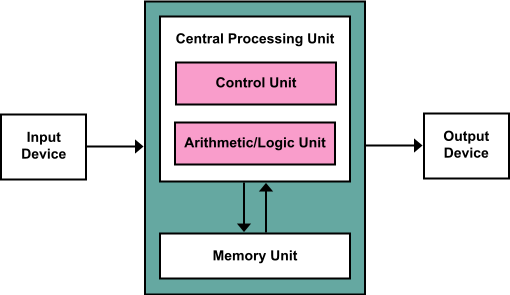
\includegraphics[width=0.6\textwidth]{Von_Neumann_Architecture.png}
\caption{Von Neumann Architecture~\cite{vonNeumannpic}}
\label{fig:vonNeumanng}
\end{figure}

We can apply the definition of Von Neumann's Architecture to further categorize two IoT edge devices:
\begin{itemize}
\item A \textbf{Micro controller unit (MCU)} is an integrated, fully capable, self-sufficient computer on a single chip. It can run a "bare metal interface", meaning that it doesn't require running an OS. Without which, it can run a single thread, or a control loop, forever. As the title of this thesis implies, MCUs are the main focus of this thesis. 
\item A \textbf{Micro processor unit (MPU)} requires support from surrounding chips that enable various functionalities like memory, interfaces, and I/O and cannot act as a stand-alone computer. The MPU, according to Von Neumann's Architecture, is just the processor unit.
\end{itemize}
While the above terms, MCU and MPU, are oftentimes used interchangeably, we want to point out the differences between these two families. It is far easier to run an OS, such as the Linux kernel~\cite{raspberrypios}, on MPU-enabled devices, such as the Raspberry Pi 4, because it is not limited to the capabilities on the chip, and can easily be extended with, i.e. more RAM~\cite{raspberrypi4}. An MCU is limited to the design and capabilities of the chip. Hence, an MPU runs with far higher processing capability and much larger applications, while MCUs are for lightweight computing where the OS if one decides to use one, is integrated on-chip. 
But because some MCUs have straightforward software drivers for more complex peripherals and more MPUs are available that have integrated peripherals on-chip, the gap between MCUs and MPUs is becoming less evident~\cite{peterson2021mcu, thornton2017mcu}.
%

\section {Processors}
When compiling software for a target platform, one must be aware of the different instruction set architectures (ISA) of the target CPUs. Listed below are the most noteworthy processor families that we came across.

\begin{itemize}
\item \textbf{ARM Cortex-M-Series}, are 32-bit RISC processors, designed for low-cost, low-power, and usually embedded in MCUs and other IoT devices~\cite{cortexm}.
\item \textbf{ARM Cortex-A-Series}, are 32-bit or 64-bit RISC processors, in contrast to the Cortex-M-Series, these processors have higher energy consumption that are built for more complex tasks such as supporting an OS~\cite{cortexa}.
\item \textbf{Tensilica Xtensa}, are 32-bit, energy-efficient, high-performance processors that build on the modular RISC architecture~\cite{xtensa}. These processors are found on MCUs.
\end{itemize}

As the description of the ARM Cortex-M and Tensilica Xtensa processors seems to fit our premise perfectly, low-cost, power-efficient and embedded in MCUs, we will focus on these types of CPUs.


\section{Market Analysis}


To find a suitable MCU that could support Linux, a market analysis had to be performed. The most relevant criteria were the following. A cheap MCU, having sizable RAM preferably more than 1MB, more than 40MHz CPU clock rate, availability in the region, and a large community. Having a sizable community can simplify development due to the availability of online resources. Furthermore with the heterogeneous nature of IoT, directing this thesis towards a smaller target audience would inevitably decrease its value. In Table~\ref{tab:market} the results are shown. Due to the countless different boards and chips that are available on the market, we grouped the chips into families defined by the manufacturers, to capture a larger picture, the column "Chip / Dev Board" reflects this. The chips were categorized into the IoT families established in Section~\ref{mcuvsmpu.ch}.

\begin{sidewaystable}[]
	\centering
	\begin{tabular}{c|c|c|c|c|c|c}

	\textbf{Manufacturer} 	& \textbf{Chip/Dev Board} & \textbf{Classification} & \textbf{CPU} & \textbf{bit} & \textbf{Clock rate} & \textbf{RAM}\\
	\hline
	\hline
	Raspberry Pi          	& Raspberry Pi 4 B	& MPU  	& ARM Cortex-A72       	& 64    	& 1.5 GHz	& 2-8 GB\\ %ok
	Raspberry Pi          	& Zero 2 W          	& MPU   	& ARM Cortex-A53       	& 64     	& 1 GHz		& 512 MB\\ %ok
	Raspberry Pi          	& Pico           		& MCU   	& ARM Cortex-M0+      & 32 	& 133 MHz 	& 264 kB\\ %ok
	\hline
	Espressif             		& ESP32              	& MCU   	& Tensilica Xtensa   	& 32		& 240 MHz	& 520 KB\\  %ok
	Espressif             		& ESP32-S2    	& MCU   	& Tensilica Xtensa   	& 32		& 240 MHz	& 320 KB\\ %ok
	Espressif             		& ESP32-C3    	& MCU   	& RISC-V       		& 32		& 160 MHz	& 400 KB\\ %ok
	Espressif             		& ESP32-S3     	& MCU   	& Tensilica Xtensa   	& 32		& 240 MHz	& 512 KB\\ %ok
	Espressif             		& ESP-EYE     		& MCU   	& Tensilica Xtensa   	& 32		& 240 MHz	& 8 MB\\ %ok
	\hline
	STMicroelectronics  	& STM32F0     	& MCU   	& ARM Cortex-M0        	& 32		& 48 MHz	& 4-32 KB\\ %ok
	STMicroelectronics  	& STM32F1     	& MCU 	& ARM Cortex-M3        	& 32		& 24-72 MHz	& 4-80 KB\\ %ok
	STMicroelectronics  	& STM32F3       	& MCU  	& ARM Cortex-M4        	& 32		& 72 MHz	& 16-80 KB\\ %ok
	STMicroelectronics  	& STM32F4       	& MCU  	& ARM Cortex-M4        	& 32		& 84-180 MHz	& 32-384 KB\\ %ok
	STMicroelectronics  	& STM32G0        	& MCU  	& ARM Cortex-M0+     	& 32		& 64 MHz	& 144 KB\\ %ok
	STMicroelectronics  	& STM32G4       	& MCU   	& ARM Cortex-M4        	& 32		& 170 MHz	& 128 KB\\ %ok
	STMicroelectronics  	& STM32L4       	& MCU   	& ARM Cortex-M4        	& 32		& 80 MHz	& 40-320 KB\\ %ok
	
	\end{tabular}
	\caption{Market analysis of available IoT edge devices}
	\label{tab:market}
\end{sidewaystable}

The Raspberry Pi modules were used as a reference, as running Linux on these boards is possible and fairly streamlined, through their own Linux distribution Raspbian~\cite{raspberrypios}. Yet, with their more capable Cortex-A processors and much larger RAM, they did not fit the criteria for this thesis.

With the exception of ESP-EYE, the insights of the market analysis, see table~\ref{tab:market}, and the realization that the required MCU on-chip RAM might not suffice for running Linux, a multitude of sales representatives of hardware manufacturers primarily of STM, were contacted. Among others, Digi-Key Electronics, Anatec AG, Avnet Silica Rothrist, Mouser Electronics, and STM personally. Questions concerning configurability and extensibility of RAM were posed with the goal of gaining expert insight. They were also specifically asked about boards such as the \code{STM32F} and \code{STM32G} series. STM personally replied with the suggestion that we should try using the \code{STM32L4} series boards and was willing to supply us with two boards visible in Figure~\ref{stm32l}. This board provided a flexible memory controller (FMC) interface and would fit our proceedings.

\begin{figure}
\centering
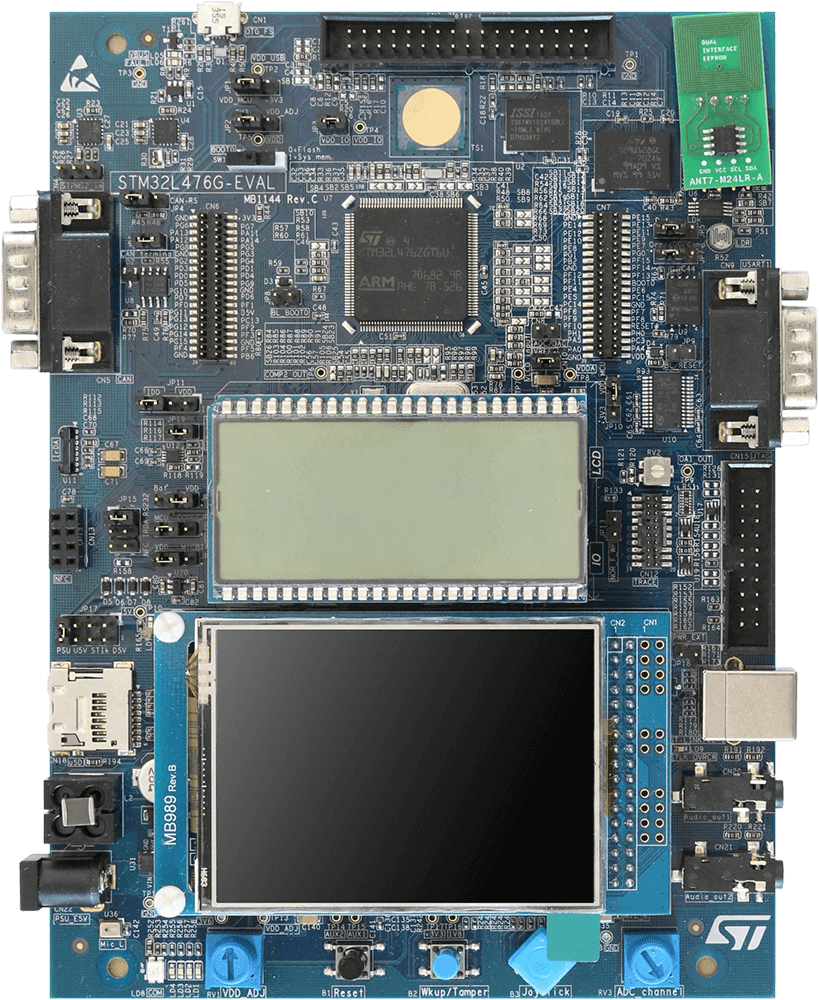
\includegraphics[width=0.6\textwidth]{stm32l476g-eval.png}
\caption{STM32L476G-Eval development board~\cite{stm32Lpic}}
\label{stm32l}
\end{figure}

\begin{figure}
\centering
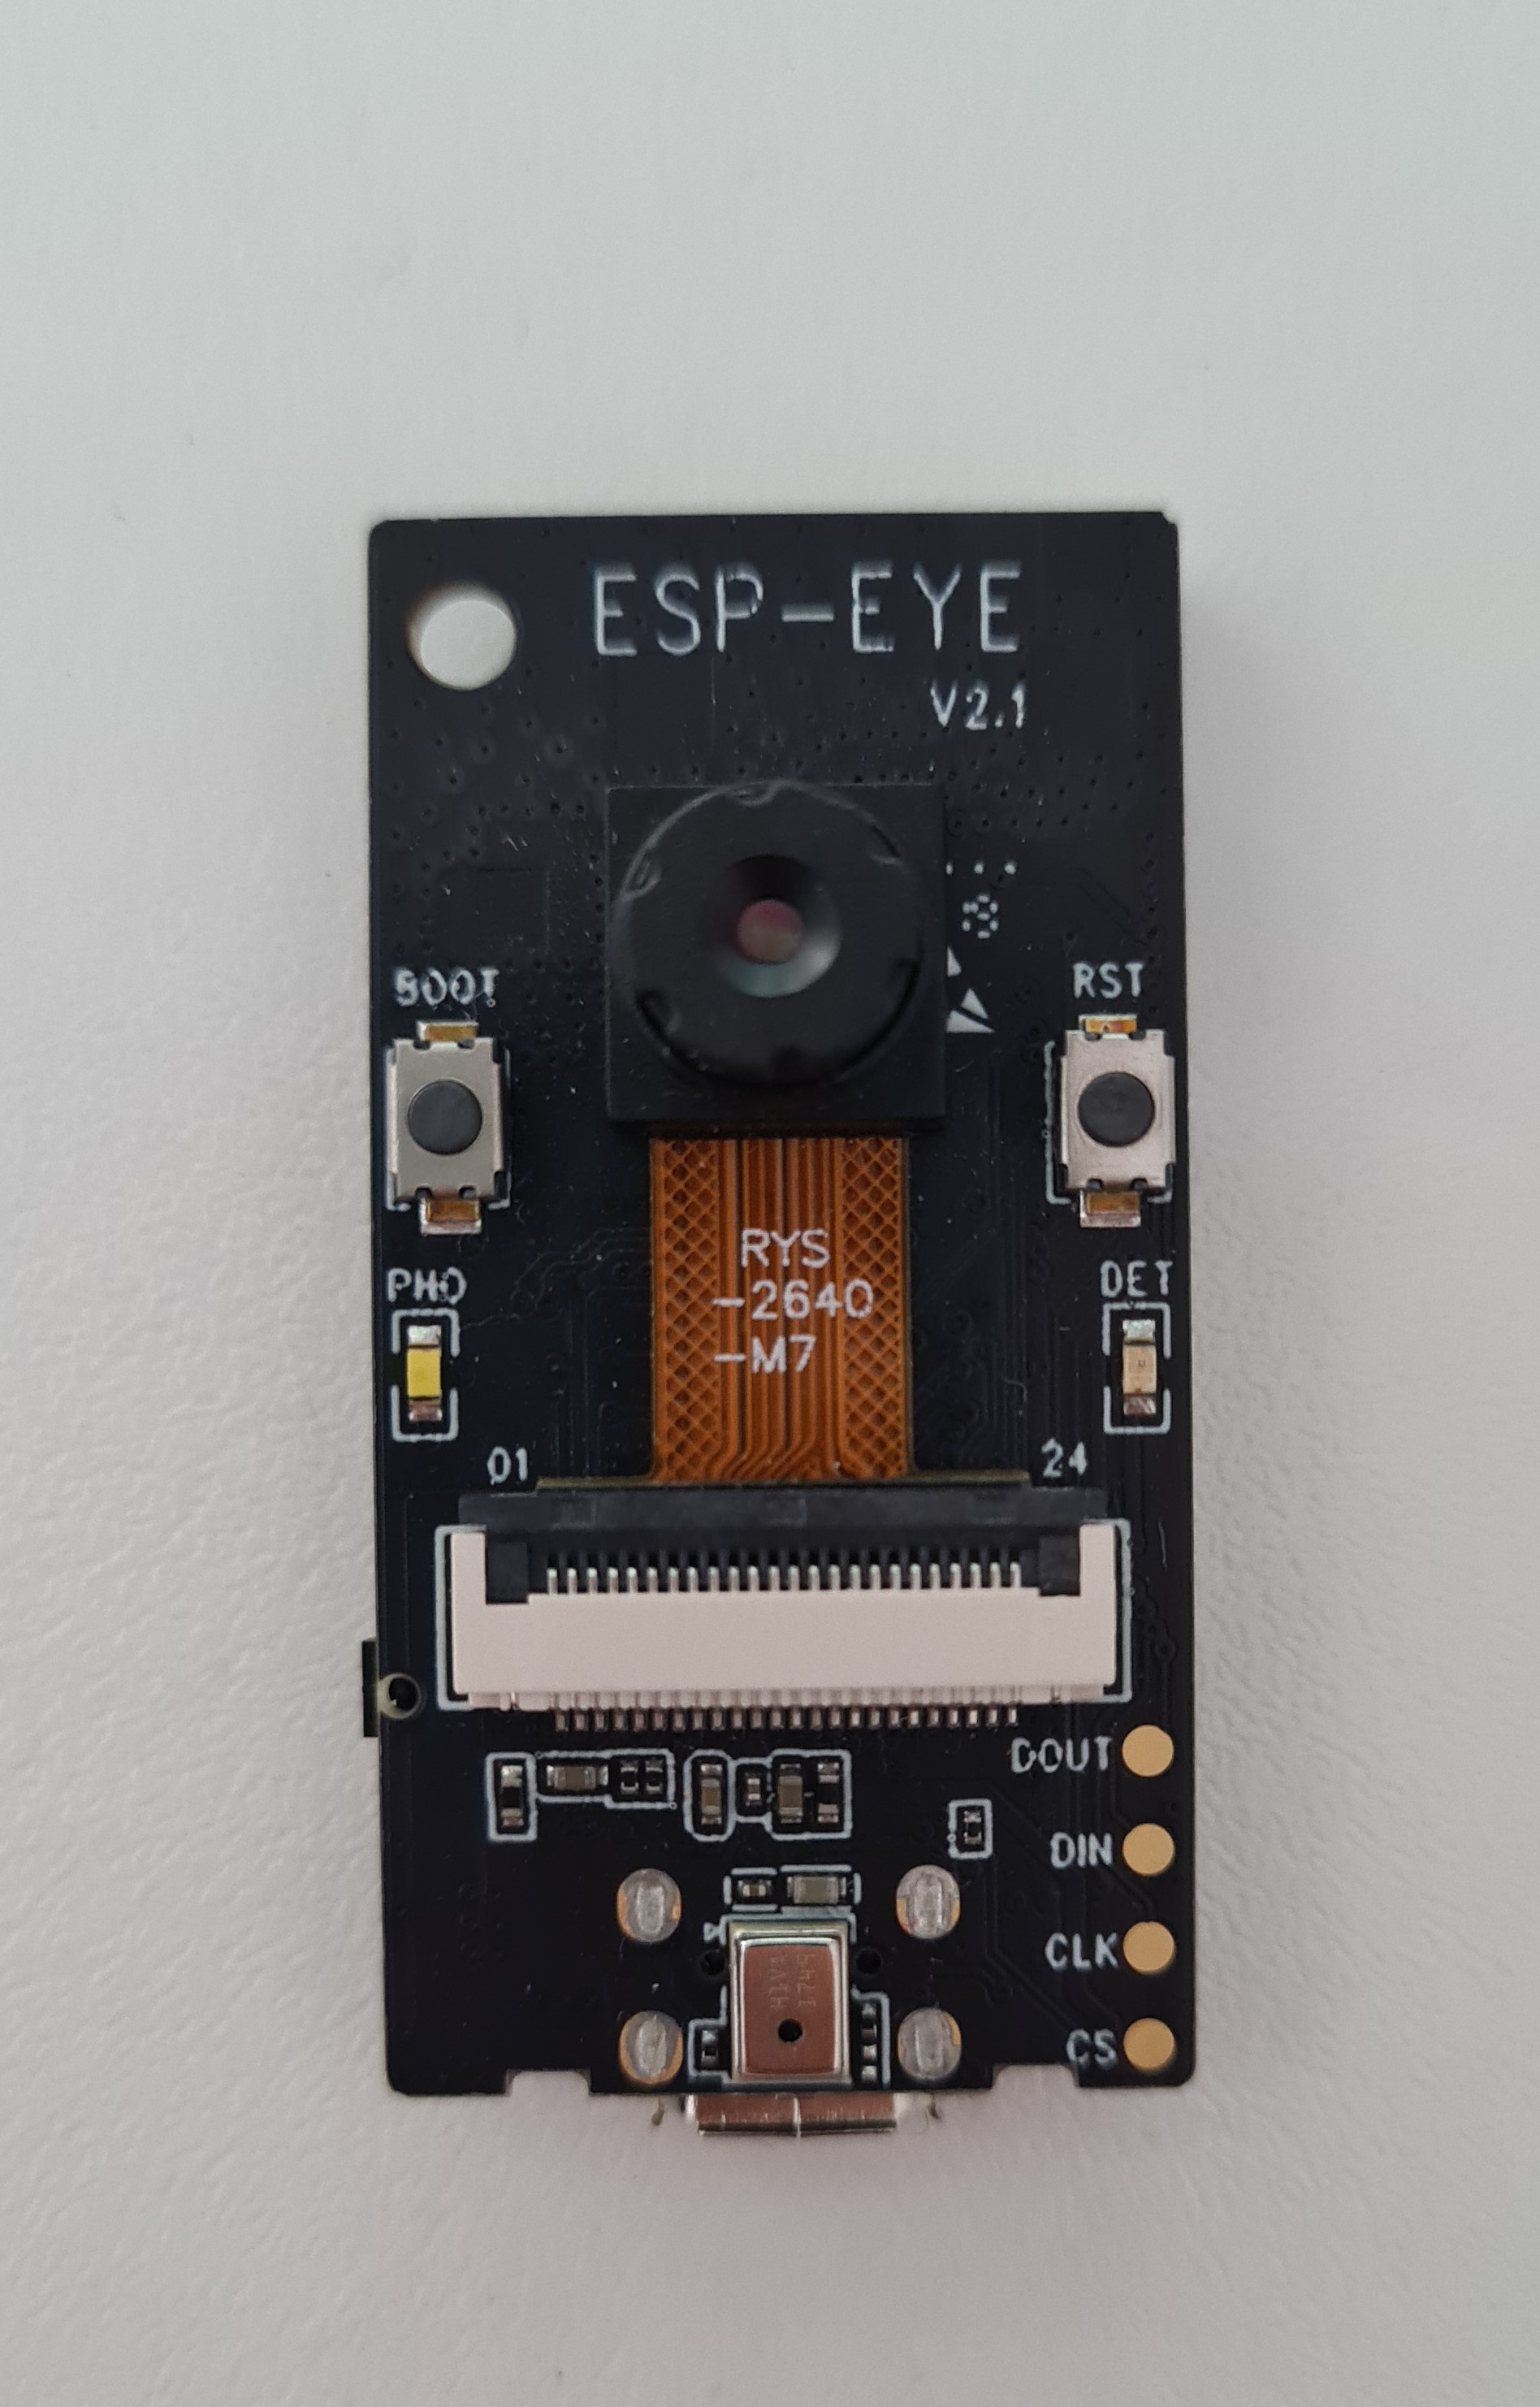
\includegraphics[width=0.4\textwidth]{ESP-EYE.jpg}
\caption{ESP-EYE}
\label{esp-eye}
\end{figure}

The second device used in this thesis is the ESP-EYE seen in Figure~\ref{esp-eye}. With its inbuilt 2MP camera and its goal to capture and process pictures as well as sound, in comparison to the other boards, it was naturally equipped with a relatively large amount of RAM.


\section{Toolchains, Cross-Compilation \& Libraries}\label{toolchains}
For compiled languages, the appropriately named toolchain combines multiple steps into a single pipeline, to produce binary or machine code. Each step in the process is a piece of software that fulfills its role or function, and hands work over to the next tool in the chain. Interpreted languages such as Python do not require compilation or toolchains, the interpreter executes, or interprets, the code directly. Since this thesis focuses on code that runs close to the hardware, interpreted languages are not considered. When compiling code a multitude of factors needs to be considered when choosing a toolchain, because they are specifically designed to work exclusively in the right circumstances. Most importantly, whether the host platform is the same as the target platform. The host is the platform on which the compilation takes place and the target on which the binaries will eventually end up running on. If the host and target platform are not the same, then we speak of cross-compilation. Another important aspect of cross-compilation is the fact that, especially in our case, the target platform may lack computing power and memory, thus compiling could be very time inefficient or simply be impossible. If compilation is mentioned, cross-compilation is implied, since the goal of this thesis is not to evaluate binary code compiled for the host system, but for the target system, the MCU edge devices. Broadly simplified toolchains work as follows.

As mentioned, the first step in a toolchain is source code compilation. Depending on the programming language the source code was written in, the compilers vary. For different compiled languages such as C and C++ different compilers are required. In our case, C is of primary concern because the Linux kernel is mostly (98.4\%) written in C~\cite{githubLinux}. From each source file that was compiled in the first step result Assembly code. Assembly code, marked with ending \code{.s}, is a set of simplified instructions and basic operations, in other words, it is a human-readable abstraction of machine code, i.e. bits.
Nowadays Assembler programming is only utilized in situations when extremely efficient management of processor activities is required, but it is still an intermediate product in the compilation. Assembly code needs to be assembled outputting object code. Finally, the object code files need to be linked with required libraries to form an, either statically or dynamically linked, executable, see section \ref{dsll}. After successful cross-compilation follows only execution on target device, which might seem like the easiest step, this is further discussed in section \ref{flashing.ch}.

For the goals of this thesis, we will be compiling, mostly, C code on the host platform operating on \code{x64} architecture for target platforms on \code{Armv7E-M} architecture. Hence cross-compilation will take place with the \code{gcc-arm-none-eabi} toolchain~\cite{gcc-arm-none-eabi}.

\subsection{Dynamically \& Statically Linked Libraries}\label{dsll}
A Library is a collection of precompiled and reusable components that hold functionality for common processes. The most common example for such a library is C's \code{stdio.h} which holds, among others, function \code{fprintf}, which simply prints characters to the console. As previously stated there are two main methods of linking such functions with the executables, we distinguish between statically linked libraries (SLL) or static libraries, and dynamically linked libraries (DLL) or shared libraries. SLL is the simplest form, as when linking, the contents of the library, specifically the required functions, are included in the executable file. On a small scale, this doesn't pose any problems, yet with more executables that are loaded into memory, each of these executables contain their own SLL. This can lead to the RAM (or ROM) being occupied by the same function multiple times. Especially when RAM is limited, as is in our case, the redundancy of the same function is not desired. DLL, on the other hand, requires only one instance of the functionality, all the executables that require this specific function can access the read-only segment of the library, therefore it can be shared. The process of sharing libraries is aided by a hardware solution, the MMU, see section~\ref{mmu.ch}.

\subsection{Buildroot }\label{buildroot.ch}
Buildroot is a tool that makes cross-compiling a complete Linux system for embedded devices easier and more automated. It runs primarily on Linux systems. Through the use of this facilitated toolchain, it creates a self-decompressing version of the Linux kernel \code{zImage}, a root filesystem, a U-boot bootloader, a root file system, and an SD card image file \code{sdcard.img}~\cite {buildroot}.

\subsection{Yocto Project \& OpenWrt}
Equivalently to Buildroot, the Yocto Project and OpenWrt are tools used for Linux cross-compilation for embedded systems. OpenWrt has a focus on Networking, the Yocto Project does not currently support MMU-less builds.~\cite{openwrt, yocto}. These tools are not used in this thesis but fill a similar role as Buildroot and are mentioned for the sake of thoroughness. 

\section{Memory Management Unit}\label{mmu.ch}
The Memory Management Unit (MMU) is hardware that is positioned between the processor and physical memory. If present, memory references from the software, through the processor, are passed through the MMU, which in turn maps these references to the actual memory, where the data being called actually resides. In more technical terms, the reference points to a virtual memory address that the MMU can translate into the physical memory address. Hence, the program running on the CPU can doesn't need to know the physical memory address. This can simplify addressing in complicated systems. Furthermore, the MMU facilitates DLL implementation. Linux's memory management system is very complicated and has grown over time, offering a growing number of features, such as \code{nommu} which means MMU-less devices, often MCUs~\cite{linuxMMU1, linuxMMU2}. While the implementation of DLL, for devices that don't contain an MMU device appears to be possible, it once again is very complicated~\cite{sharedLibnoMMU}. There exist Linux variations that are tailored for MMU-less devices, see section~\ref{uclinux.ch}.

\section{The Linux Kernel}
The Linux Kernel (Linux) was initially created, by Linus Torwalds, in 1991 for i368 based PCs. After its initial appearance, it quickly gained traction among developers and was licensed under GNU General Public License (GPL) as free OSS~\cite{linuxlicense}. At the current time, Linux supports all kinds of different target architectures and dominates that IoT market~\cite{sabri2017comparison}.


\subsection{$\mu$Clinux}\label{uclinux.ch}
The open-source nature of Linux made it possible to fork the source code and modify it according to one's needs. One such project is the $\mu$Clinux, which was specifically created to target MMU-les microcontrollers. Its hardware-dependent, such as physical memory, and independent, such as virtual memory, code is distinct. Using the given instructions, the hardware-specific portion may be altered for a number of CPUs, hence the OS is modifiable. The system supports both user space and kernel space, and switching between the two may be done using system calls. It is possible to develop in a multi-threading environment using POSIX thread libraries. Neither a virtual memory model nor a memory protection unit exists, but functions can be used to dynamically allocate memory, hence DLL is possible. It features a complete TCP/IP stack that may be swapped out for a lighter stack like uIP or lwIP~\cite{dunkels2003full}. But, in comparison to other IoT edge device OSs, as seen in Section~\ref{iotos.ch}, $\mu$Clinux has a far larger footprint than other IoT OSes~\cite{gaur2015operating}. $\mu$Clinux was eventually discontinued as a standalone fork and was reintroduced into the mainline Linux kernel. With the official emailing list gone quiet and its webpage only visible through web archives, and the last official update published in May of 2016~\cite{uclinux.org}. Other entities appear to have forked and maintained it further down the line, such as emcraft~\cite{emcraft, emuClinux}, with the last commits on December 2017, one year later. The last remaining verifiable remnants appear to be pointing toward a "small C library for developing embedded Linux systems" called uclibc-ng~\cite{uclibc-ng}, which could prove useful.

\subsection{Device Trees}
The device tree is a data structure that describes the hardware, that is locally available, for the device we want to port Linux to. The device tree is the dynamic solution for the problem that the CPU must know its environment. 

\section{U-Boot}
"Das U-Boot" is an open-source boot loader used predominantly in embedded devices. Its main focus is to load the OS kernel into the main memory. It supports a wide variety of IoT development boards~\cite{u-boot-doc}. Yet again, as is common in the IoT ecosystem, there is a multitude of U-Boot forks, the original and the one that appears to be maintained and updated most frequently is made available by denx, while the previously mentioned emcraft has their own~\cite{emUboot}. When not otherwise mentioned, when U-Boot is mentioned we are referring to U-Boot maintained by denx~\cite{u-boot}.

\section{QEMU}\label{qemu.ch}
Primarily a general-purpose machine virtualizer and emulator, QEMU has a variety of applications. In this thesis we will use it to emulate a system, thus creating a virtual replica of an MCU, including the CPU, memory, and simulated peripherals, in order to run a compiled version of Linux. The CPU may operate in this mode entirely emulated or in conjunction with a hypervisor like Kernel-based Virtual Machine (KVM), Xen, Hax, or Hypervisor. Equivalently to the cross-compilation process that was discussed in section \ref{toolchains}, the "user mode emulation," allows QEMU to run programs that were built for the target CPU, on our host CPU~\cite{qemu}.

\section{JuiceVM}
JuiceVM is a found on GitHub, that started in 2020, with only three visible contributors~\cite{juicevm}. Self-described, it is a small RISC-V Virtual Machine (VM), capable of running on just a few hundred KB of RAM. Unter its demonstration projects it shows that it can boot Linux, which is why this thesis found interest in the project. While it only provides precompiled binaries, and the source code not being visible to the public, it can still provide the required functionalities that we seek.

\section {STM Tools}\label{stm.ch}
Specifically, two STM provided tools were used in this thesis, STM32CubeProgrammer and STM32CubeIDE 1.9.0. The former provides functionality to connect to the STM boards through the ST-LINK/V2 interface, enables easy flashing capabilities through a GUI, and information on the state RAM and ROM. The latter is an IDE designed for embedded programming that facilitates the creation of projects, the initialization of various libraries, configuration of the chip's I/O peripherals, compilation, and debugging. Additionally, it is possible to flash a connected STM device directly through the IDE.

\section{Miscelanous Tools}
Various different utilities and tools are required that help achieve certain goals, here the most noteworthy are listed. PuTTY is an open-source software developed for Windows OS that, among others, provides SSH and serial port connections. With this tool, a connection to the devices can be established and consoles viewed. Docker is a platform providing virtualization functionalities, it is used to build a Linux-based container, in which the compilations will be executed. By providing great portability it allows future researchers to use the built container. Disk Imager is a small windows utility that enables the flashing of SD cards with \code{.img} files. \code{esptool.exe} is a command line utility tool that will allow us to flash ESP32 chips with binaries, mainly the ESP-EYE.
